% https://tex.stackexchange.com/questions/51757/how-can-i-use-tikz-to-make-standalone-svg-graphics
\documentclass{standalone}
\usepackage[svgnames]{xcolor} % Enabling colors by their 'svgnames'
\usepackage{tikz}
\usetikzlibrary{calc}
\usepackage{amsmath,amsfonts,amsthm}
\usepackage{physics}

\begin{document}
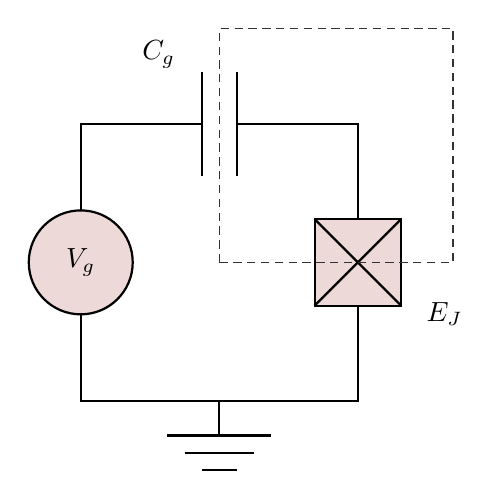
\begin{tikzpicture}[scale=2.2]
    
    \filldraw[thick, fill=DarkRed!15] (0,0) circle [radius=0.3];
    \node at (0,0) {\normalsize $V_g$}; 
    
    \draw[thick] (0,0.3) -- (0,0.8) -- (0.7,0.8); %Top left corner
    
    %Capacitor
    \draw[thick] (0.7, 0.5) -- (0.7, 1.1); %Left plate
    \draw[thick] (0.9, 0.5) -- (0.9, 1.1); %Right plate
    % \node at (0.8,1.35) {\footnotesize $C_g$}; 
    \node at (0.45,1.2) {\normalsize $C_g$}; 
    
    \draw[thick] (0.9,0.8) -- (1.6,0.8) -- (1.6,0.25); %Top right corner
    
    %Josephson junction.
    \filldraw[thick, fill=DarkRed!15] (1.35,-0.25) rectangle (1.85, 0.25); %Box
    \draw[thick] (1.35, 0.25) -- (1.85,-0.25); %Down diagonal
    \draw[thick] (1.35,-0.25) -- (1.85, 0.25); %Up diagonal
    % \node at (2.1,0) {\footnotesize $E_J$}; 
    \node at (2.1,-0.3) {\normalsize $E_J$}; 
    
    \draw[thick] (1.6,-0.25) -- (1.6,-0.8) -- (0,-0.8) -- (0,-0.3); %Lower part of the CPB.
    
    %Ground
    \draw[thick] (0.8,-0.8) -- (0.8,-1);
    \draw[thick] (0.5,-1) -- (1.1,-1);
    \draw[thick] (0.6,-1.1) -- (1,-1.1);
    \draw[thick] (0.7,-1.2) -- (0.9,-1.2);
    
    %Island
    \draw[semithick, densely dashed, color=Black!80] (0.8, 0) rectangle (2.15, 1.35);
    
\end{tikzpicture}
\end{document}

